
\subsection{Genus}
\index{genus|(}%
Termin genus został wymyślony przez Clebscha około 1864 roku (w~,,Über die Anwendung der Abelschen Functionen in der Geometrie'', jak można przeczytać w~przypisie do pracy ,,Development of the concept of homotopy'' Rii Vanden Eynde) i początkowo oznaczał po prostu liczbę dziur w~powierzchni.
Jak piszą Burde, Zieschang, Heusener \cite[s. 20]{burde2014}, \emph{,,the notion of the genus was first introduced by H. Seifert in \cite{seifert1935}, it holds a central position in knot theory''}; zbadamy więc teraz bliżej ten geometryczny niezmiennik węzłów.
(Nie pamiętamy, czemu ta podsekcja znajduje się akurat tutaj, ale chyba nie jest to najgorsze miejsce dla niej.)

Zaczniemy od starego twierdzenia, które klasyfikuje powierzchnie domknięte.

\begin{proposition}
    Niech $S$ będzie powierzchnią domkniętą.
    Wtedy dokładnie jedno zdanie z~poniższych jest prawdziwe:
    \begin{enumerate}[leftmargin=*]
        \itemsep0em
        \item $S$ jest orientowalna, sumą spójną $g \ge 0$ torusów
        \item $S$ jest nieorientowalna, sumą spójną $k \ge 1$ rzeczywistych płaszczyzn rzutowych.
    \end{enumerate}
    Liczby $g$ lub $k$ są wyznaczone jednoznacznie. % , to znaczy jeśli coś jest sumą spójną $g_1$ lub $g_2$ torusów, to $g_1 = g_2$ i podobnie dla płaszczyzn rzutowych).
\end{proposition}

Sferę traktujemy dla wygody jako sumę spójną $g = 0$ torusów.
Wtedy sumę spójną $g$ torusów możemy wyobrazić sobie jako sferę, do której doklejono $g$ rączek.
(Suma spójna torusa i~płaszczyzny rzutowej jest tym samym, co suma spójna trzech płaszczyzn rzutowych -- wykazanie tego jest jednym z kroków w klasyfikacji powierzchni.)

\begin{definition}[genus powierzchni]
    Niech $S$ będzie orientowalną powierzchnią będącą sumą spójną $\genus$ torusów.
    Liczbę $\genus$ nazywamy genusem powierzchni $S$.
\end{definition}

Podobna charakteryzacja istnieje dla powierzchni z~brzegiem.
Każdy taki obiekt jest homeomorficzny z~sumą spójną $g$ torusów, w~których wydrążono pewną liczbę otworów: tyle, ile składowych spójności ma brzeg powierzchni.
W~przypadku powierzchni Seiferta mamy do czynienia z jednym otworem.

Definiujemy jeszcze jeden klasyczny niezmiennik powierzchni: charakterystykę Eulera-Poincarégo, odkrytą najpierw dla wielościanów platońskich w 1537 roku przez Francesco Maurolico i wiele lat później przez Eulera dla wielościanów wypukłych.
(Obecnie wyprowadza się ją z homologii/algebry homologicznej, ale darujemy to sobie).

\begin{definition}[charakterystyka Eulera]
\index{charakterystyka Eulera}%
    Niech $S$ będzie domkniętą powierzchnią orientowalną.
    Po striangulowaniu, składa się z $k_0$ wierzchołków, $k_1$ krawędzi oraz $k_2$ ścian.
    Wielkość
    \begin{equation}
        \chi = k_0 - k_1 + k_2
    \end{equation}
    jest niezmiennikiem powierzchni, zwanym charakterystyką Eulera.
\end{definition}

Definicja ta nie jest wygodna podczas ręcznych obliczeń.
Mamy za to:

\begin{proposition}
    Charakterystykę Eulera powierzchni jednoznacznie wyznaczają cztery reguły, gdzie stale $S_1, S_2$ są pewnymi powierzchniami, zaś $S$ jest dyskiem:
    \begin{itemize}
        \item $\chi(S) = 1$,
        \item $\chi(S_1 \sqcup S_2) = \chi(S_1) + \chi(S_2)$,
        \item Jeśli $S_2$ powstaje z $S_1$ przez dołączenie paska, to $\chi(S_2) = \chi(S_1) - 1$,
        \item Jeśli $S_2$ powstaje z $S_1$ przez dołączenie dysku do całej składowej spójności brzegu, to $\chi(S_2) = \chi(S_1) + 1$.
    \end{itemize}
\end{proposition}

Genus oraz charakterystyka Eulera są ze sobą związane:

\begin{proposition}
    Niech $S$ będzie powierzchnią o genusie $\genus$ i $\mu$ składowych spójności brzegu.
    Wtedy zachodzi równość
    \begin{equation}
        \chi = 2 - \mu - 2\genus.
    \end{equation}
\end{proposition}

Nas interesują głównie powierzchnie Seiferta węzłów:
\index{powierzchnia!Seiferta}%

\begin{proposition}
\label{prp:seifert_euler_characteristics}%
    Niech $D$ będzie diagramem o $b$ skrzyżowaniach pewnego węzła $K$, z którego algorytm Seiferta produkuje $d$ okręgów.
    Wtedy $\chi(M_D) = d - b$.
\end{proposition}

Można przeczytać o tym w \cite[s. 82]{murasugi1996}.

\begin{proof}
    W~dowodzie faktu \ref{prp:seifert_exists} widzieliśmy, że liczba skrzyżowań $b$ jest jednocześnie liczbą pasków doklejonych do dysków.
    Bezpośredni rachunek pokazuje, że wtedy $k_0 = 4b$, $k_1 = 6b$ oraz $k_2 = b+d$.
    Wynika stąd, że $\chi = 4b - 6b + b + d = d - b$.
\end{proof}

Reszta tej podsekcji nie jest wymagana do zrozumienia macierzy Seiferta, przyjrzymy się genusowi jako obiektowi ciekawemu samemu w sobie.

\begin{definition}[3-genus]
    Niech $K$ będzie węzłem.
    Wśród wszystkich powierzchni Seiferta węzła $K$ istnieje co najmniej jedna o minimalnym genusie, jej genus nazywamy 3-genusem węzła $K$ i oznaczamy także przez $\genus$.
\end{definition}

Jeżeli nie powoduje to nieporozumień, zamiast 3-genus można pisać po prostu genus.

\begin{proposition}
\label{prp:genus_detects_unknot}%
    Węzeł $K$ jest niewęzłem wtedy i tylko wtedy, gdy $\genus K = 0$.
\end{proposition}

,,Genus wykrywa niewęzły''.

\begin{proof}
    Niech $K$ będzie węzłem o genusie $0$.
    Z~charakteryzacji powierzchni wynika, że jego powierzchnia Seiferta to suma spójna $0$ torusów, to znaczy kula z tyloma otworami, ile $K$ ma ogniw.
    Innymi słowy, powierzchnią Seiferta węzła $K$ jest dysk, którego brzeg stanowi niewęzeł.
    To pokazuje, że implikacja w lewo jest prawdziwa.

    Implikacja w prawo jest oczywista.
\end{proof}


\subsubsection{Ograniczanie genusu z dołu}
Znalezienie 3-genusu dowolnego węzła sprawia te same trudności, co wyznaczenie jego liczby gordyjskiej.
Dowolna powierzchnia Seiferta zadaje ograniczenie z góry.
Z dołu 3-genus można szacować przy użyciu wielomianu Alexandera:
\index{wielomian!Alexandera}%

\begin{proposition}
\label{prp:alexander_genus}%
    Niech $K$ będzie węzłem.
    Wtedy $\operatorname{span} \alexander_K(t) \le 2\genus(K)$.
\end{proposition}

Fakt ten znalazłem w podręczniku Murasugiego \cite[s. 131]{murasugi96}.

\begin{proof}
    Załóżmy, że $F$ jest powierzchnią Seiferta węzła $K$ o genusie $g$.
    Wtedy macierz Seiferta powstała z $F$ jest stopnia $2g$, więc żaden ze składników jej wyznacznika nie może mieć stopnia (jako wielomian) większego niż $2g$.
\end{proof}

To dolne ograniczenie jest realizowane przez pewną powierzchnię Seiferta dla każdego pierwszego węzła o~co najwyżej 11 skrzyżowaniach poza siedmioma wyjątkami: 11n42, 11n67, 11n97 ($g = 2$), 11n34, 11n45, 11n73 oraz 11n152 ($g = 3$).
% warto byłoby dodać jakiś kod pozwalający sprawdzić, czemu akurat te węzły

\begin{proposition}
    Niech $K$ będzie węzłem, zaś $M$ jego macierzą Seiferta.
    Równość $\operatorname{span} \alexander_K(t) = 2\genus(K)$ zachodzi wtedy i tylko wtedy, gdy wyznacznik $\det M \neq 0$ jest niezerowy.
\end{proposition}

Floer zdefiniował w~\cite{floer90} przestrzeń wektorową nazywaną teraz homologią Floera, jest ona wyposażona w~endomorfizm parzystego stopnia, który powstaje z 2-wymiarowej klasy homologii reprezentowanej przez powierzchnię Seiferta.
%~kanoniczną gradację modulo $2$ oraz
\index{homologia!Floera}
Ta homologia rozkłada się na sumę prostą przestrzeni własnych wyróżnionego endomorfizmu, ich charakterystyki Eulera są współczynnikami wielomianu Alexandera.
Pozwala to na dokładniejsze szacowanie genusu węzła, patrz prace Ozsvátha, Szabó \cite{szabo03} i Ghigginiego \cite{ghiggini08}.
\index[persons]{Ghiggini, Paolo}%
\index[persons]{Ozsváth, Peter}%
\index[persons]{Szabó, Zoltán}%




\subsubsection{Ograniczanie genusu z góry}
Z góry genus ograniczony jest przez kilka klasycznych niezmienników numerycznych.
Zanim to pokażemy, przytoczymy techniczny lemat udowodniony przez Yamadę \cite{yamada87}.
\index[persons]{Yamada, Shuji}%

\begin{proposition}
\index{indeks warkoczowy}%
\label{prp:seifert_circles_braid}%
    Niech $L$ będzie splotem, zaś $\operatorname{s} L$ minimalną liczbą okręgów Seiferta, które dostajemy ze wszystkich możliwych diagramów splotu $L$.
    Wtedy $\operatorname{s} L = \braid L$ jest równe indeksowi warkoczowemu.
\end{proposition}

Powyższe stwierdzenie występuje bez dowodu (bez?) w \cite[s. 17]{kawauchi96}.
Zmyślny dowód Yamady polega na zmianie rzutu tak, by nie zmienić liczby okręgów Seiferta.

\begin{proposition}
    Niech $L$ będzie splotem.
    Wtedy $\crossing L - \braid L - \operatorname{\mu} L + 2 \ge 2 \genus L$.
\end{proposition}

\begin{proof}
    Ustalmy minimalny diagram $D$ dla splotu $L$ i zastosujmy do niego algorytm Seiferta.
    Dostaniemy tak $s$ okręgów Seiferta oraz powierzchnię o genusie $g$.
    Fakt \ref{prp:seifert_euler_characteristics} mówiący, że $\chi = s - c$, można przekształcić do
    \begin{equation}
        g = \frac{c + 2 - s - \mu(K)}{2}.
    \end{equation}
    Z~minimalności diagramu wynika, że $c = \crossing L$.
    Fakt \ref{prp:seifert_circles_braid} mówi, że $s \ge \braid L$.
    Nierówność $g \ge \genus L$ wynika z~definicji genusu.
    Z powyższych rozważań wynika, że
    \begin{equation}
        \crossing L + 2 \ge 2 \genus L + \braid L + \operatorname{\mu} L,
    \end{equation}
    a to jest równoważnie nierówności, której prawdziwości dowodzimy.
\end{proof}

\begin{corollary}
\index{indeks skrzyżowaniowy}%
\label{cor:crossing_genus}%
    Niech $K$ będzie węzłem.
    Wtedy $\crossing K \ge 2 \genus K$.
\end{corollary}

% koniec psot




\subsubsection{Genus a rozkład na sumę węzłów pierwszych}

\begin{proposition}
    \label{prp:genus_of_sum}
    Jeśli $K_1, K_2$ są węzłami, to $\genus (K_1 \shrap K_2) = \genus (K_1) + \genus (K_2)$.
\end{proposition}

Poniższy dowód pochodzi od Schuberta (\cite{schubert49}), został tylko zapisany we współczesnym języku.
\index[persons]{Schubert, Horst}%
Przebiega w dwóch etapach: najpierw pokazuje się, że genus sumy nie jest większy od sumy genusów składników, a następnie, że nie jest od niej mniejszy.

\begin{proof}
    Pokażemy najpierw, że $\genus (K_1 \# K_2) \le \genus (K_1) + \genus (K_2)$.
    Wybierzmy powierzchnie Seiferta $M_1$ oraz $M_2$ dla $K_1$ oraz $K_2$ o~minimalnym genusie.
    Suma $K_1 \shrap K_2$ powstaje z~$K_1$ oraz $K_2$, podobnie jest z~powierzchniami Seiferta:
\begin{comment}
    \begin{figure}[H]
        \centering
        \begin{minipage}[b]{.48\linewidth}
        \[
            \LargeGenusProofA \longrightarrow \LargeGenusProofB
        \]
        \subcaption{suma węzłów}
        %
        \end{minipage}
        \begin{minipage}[b]{.48\linewidth}
        \[
            \LargeGenusProofC \longrightarrow \LargeGenusProofD
        \]
        \subcaption{suma powierzchni}
        \end{minipage}
    \end{figure}
\end{comment}

    Skoro $M_{\#}$ powstaje z~$M_1 \sqcup M_2$ przez dołączenie paska do brzegu, mamy
    \begin{equation}
        \chi(M_{\#}) = \chi(M_1 \sqcup M_2) - 1 = \chi(M_1) + \chi(M_2)-1,
    \end{equation}
    a~przez to
    \begin{equation}
        \genus (M_{\#}) = \frac{1-\chi(M_{\#})}{2} =
        \frac{1-\chi(M_1)}{2} + \frac{1-\chi(M_2)}{2}
        % = %g(M_J)+g(M_K)
        = \genus(K_1) + \genus(K_2).
    \end{equation}
    To kończy dowód pierwszej nierówności.

    Pokażemy jeszcze, że $\genus (K_1 \# K_2) \ge \genus (K_1) + g(K_2)$.
    Zaczynamy od powierzchni Seiferta $M_{\#}$ dla $K_1 \# K_2$ o~minimalnym genusie $\genus (M_{\#})$ równym $\genus (K_1 \# K_2)$.
    Poprzez wykonanie chirurgii na powierzchni, możemy przyjąć specjalną postać jak w~poprzednim dowodzie:
\begin{comment}
    \[
        \LargeGenusProofD
    \]
\end{comment}

    Usunięcie paska daje powierzchnie Seiferta dla $M_1$ oraz $M_2$ takie, że
    \begin{equation}
        \genus(M_1) + \genus(M_2) = \genus(M_{\#}) = \genus(K_1 \# K_2).
    \end{equation}
    Oznacza to, że $\genus(K_1) + \genus(K_2) \le \genus(M_1) + \genus(M_2) = \genus(K_1 \# K_2)$ i~mamy równość.
\end{proof}

Jesteśmy wreszcie w~stanie podać ,,prawdziwy dowód'' faktu \ref{first_time_sum_is_trivial}.

\begin{corollary}
\label{cor:connected_sum_no_inverses}%
    Jeśli suma spójna dwóch węzłów jest niewęzłem, to oba składniki także nim są.
\end{corollary}

Powrócimy teraz do węzłów pierwszych.
\index{węzeł!pierwszy}%

\begin{proposition}
    Niech $K$ będzie węzłem.
    Jeśli $\genus (K) = 1$, to $K$ jest węzłem pierwszym.
\end{proposition}

\begin{proof}
    Załóżmy nie wprost, że węzeł $K = K_1 \# K_2$ jest sumą dwóch nietrywialnych węzłów.
    Z~faktu \ref{prp:genus_of_sum} wynika wtedy, że $g(K) = g(K_1) + g(K_2)$.
    Zatem jeden z węzłów $K_1, K_2$ ma genus zero i jest trywialny, wbrew naszemu założeniu.
\end{proof}

Implikacja odwrotna jest fałszywa: pięciolistnik jest pierwszy, ale jego genus wynosi $2$.
Spośród 2977 węzłów pierwszych do 12 skrzyżowań, tylko 23 posiada genus równy jeden.
Są to: $3_{1}$, $4_{1}$, $5_{2}$, $6_{1}$, $7_{2}$, $7_{4}$, $8_{1}$, $8_{3}$, $9_{2}$, $9_{5}$, $9_{35}$, $9_{46}$, $10_{1}$, $10_{3}$, $11a_{247}$, $11a_{343}$, $11a_{362}$, $11a_{363}$, $11n_{139}$, $11n_{141}$, $12a_{803}$, $12a_{1166}$ oraz $12a_{1287}$.
% ZWERYFIKOWANO: funkcja genus_prime

\begin{proposition}
    Każdy węzeł można zapisać jako suma spójna pewnej liczby węzłów pierwszych.
    Niewęzeł jest sumą pustej rodziny węzłów.
\end{proposition}

\begin{proof}
    Dowodzimy przez indukcję względem genusu $\genus (K)$.
    Przypadek bazowy $\genus (K) = 0$ jest oczywisty, gdyż wtedy $K$ to niewęzeł.
    Załóżmy więc, że fakt zachodzi dla węzłów $J$ genusu co najwyżej $n$.
    Niech $K$ będzie genusu $n + 1$.

    Jeśli $K$ jest pierwszy, nie ma czego dowodzić.
    W przeciwnym razie jest równoważny z~$J_1 \shrap J_2$, gdzie $J_1$ i~$J_2$ są nietrywialne.
    Mamy $\genus (J_1) + \genus (J_2) = g(K)$ oraz $\genus(J_1), \genus(J_2) \ge 1$.
    Zatem $\genus(J_1), \genus(J_2) \le n$.
    Na mocy hipotezy indukcyjnej, $J_1$ oraz $J_2$ są równoważne sumom
    \[
        J_1 \cong K_1 \# \cdots \# K_s, \qquad
        J_2 \cong K_{s+1} \# \cdots \# K_r,
    \]
    gdzie $K_i$ są pierwsze.
    Zatem $K$ jest równoważny z~$K_1\#\cdots\# K_r$, co kończy dowód.
\end{proof}

Nasz aparat matematyczny jest niedostatecznie rozwinięty, by móc udowodnić jedyność rozkładu.

\begin{theorem}[Schubert, 1949]
    Każdy nietrywialny węzeł rozkłada się na węzły pierwsze.
    Rozkład jest, z dokładnością do kolejności składników, jednoznaczny.
\index{węzeł!pierwszy}%
\end{theorem}

Schubert podał geometryczny dowód oparty o powierzchnie Seiferta; wyraził go w języku PL-rozmaitości (\cite{schubert49}), ale niedużym wysiłkiem można dokonać adaptacji do gładkiego świata.
\index[persons]{Schubert, Horst}%
Praca Schuberta korzysta z twierdzenia Alexandera, że 2-sfera w przestrzeni $\R^3$ ogranicza dysk, i jego odpowiednika dla torusów w $S^3$.

Hashizume \cite{hashizume58} rozszeszył wyniki Schuberta do splotów.
\index[persons]{Hashizume, Yoko}%
% TODO trzeba wspomnieć, że to wymaga adaptacji definicji sumy spójnej, bo wcześniej dopuszczaliśmy tylko węzły jako składniki. Remedium = Kawauchi.

\begin{proposition}
\label{prp:infinitely_many_prime_knots}%
    Istnieje nieskończenie wiele węzłów pierwszych.
\end{proposition}

\begin{proof}
    Pokażemy, że wszystkie węzły $(2n+2)_1$ są pierwsze, gdzie $n \ge 1$.
    Istotnie, algorytm Seiferta zastosowany do diagramu tego węzła wyprodukuje $2n+1$ okręgów.
\begin{comment}
    \[
        \begin{tikzpicture}[baseline=-0.65ex,scale=0.06]
        \begin{knot}[clip width=7, flip crossing/.list={1,4,5},end tolerance=1pt]
            \node at (0,10) {$\cdots$};
            \strand[semithick] (-30, -5) -- (-5, -5);
            \strand[semithick]  (5, -5) -- (30, -5);
            \strand[semithick,latex-]  (-30,-15) -- (-5,-15);
            \strand[semithick]  (5,-15) -- (30,-15);

            \strand[semithick] (-5, -15) [in=down, out=right] to (5, -10) [in=right, out=up] to (-5, -5);
            \strand[semithick] (5, -15) [in=down, out=left] to (-5, -10) [in=left, out=up] to (5, -5);

            % zewnętrzne obręcze -- lewa strona
            \strand[semithick] (-30, 15) to [out=left, in=up]   (-45, 0);
            \strand[semithick] (-30,-15) to [out=left, in=down] (-45, 0);
            \strand[semithick] (-30,  5) to [out=left, in=up]   (-35, 0);
            \strand[semithick] (-30, -5) to [out=left, in=down] (-35, 0);

            % zewnętrzne obręcze -- prawastrona
            \strand[semithick] (30, 15) to [out=right, in=up]   (45,0);
            \strand[semithick] (30,-15) to [out=right, in=down] (45,0);
            \strand[semithick] (30,  5) to [out=right, in=up]   (35,0);
            \strand[semithick] (30, -5) to [out=right, in=down] (35,0);

            % jak w~drugim ruchu Reidemeistera - górny warkocz, lewy
            \strand[semithick] (-30, 15) [in=left, out=right] to (-20,  5);
            \strand[semithick] (-30,  5) [in=left, out=right] to (-20, 15);
            \strand[semithick] (-10, 15) [in=right, out=left] to (-20,  5);
            \strand[semithick] (-10,  5) [in=right, out=left] to (-20, 15);

            % jak w~drugim ruchu Reidemeistera - górny warkocz, prawy
            \strand[semithick] (30, 15) [in=right, out=left] to (20,  5);
            \strand[semithick] (10, 15) [in=left, out=right] to (20,  5);
            \strand[semithick] (30,  5) [in=right, out=left] to (20, 15);
            \strand[semithick] (10,  5) [in=left, out=right] to (20, 15);
        \end{knot}
        \end{tikzpicture}
        \longrightarrow
        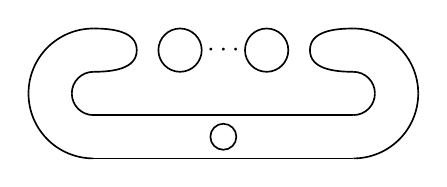
\begin{tikzpicture}[baseline=-0.65ex,scale=0.055]
            \node at (0,10) {$\cdots$};
            \draw[semithick] (-30,  -5) -- (30, -5);
            \draw[semithick] (-30, -15) -- (30,-15);

            \draw[semithick] (0,-10) circle (3);

                % zewnętrzne obręcze -- lewa strona
            \draw[semithick] (-30, 15) to [out=left, in=up]   (-45, 0);
            \draw[semithick] (-30,-15) to [out=left, in=down] (-45, 0);
            \draw[semithick] (-30,  5) to [out=left, in=up]   (-35, 0);
            \draw[semithick] (-30, -5) to [out=left, in=down] (-35, 0);

                % zewnętrzne obręcze -- prawastrona
            \draw[semithick] (30, 15) to [out=right, in=up]   (45,0);
            \draw[semithick] (30,-15) to [out=right, in=down] (45,0);
            \draw[semithick] (30,  5) to [out=right, in=up]   (35,0);
            \draw[semithick] (30, -5) to [out=right, in=down] (35,0);

            \draw[semithick] (-30, 15) to [out=right, in=up] (-20,10);
            \draw[semithick] (-30,  5) to [out=right, in=down] (-20,10);

            \draw[semithick] (30, 15) to [out=left, in=up] (20,10);
            \draw[semithick] (30,  5) to [out=left, in=down] (20,10);

            \draw[semithick] (-10, 10) circle (5);
            \draw[semithick] (10,  10) circle (5);
        \end{tikzpicture}
    \]
\end{comment}
    Wynika stąd, że genus wynosi $\frac 12 (1 - (1+2n) + (2+2n)) = 1$, ponieważ wyznacznik ma wartość $4n+1$,
    węzły $(2n+2)_1$ nie są trywialne i~są parami różne.
\end{proof}




\subsubsection{Genus kanoniczny, genus wolny}
% DICTIONARY;free;wolny;genus
% DICTIONARY;canonical;kanoniczny;genus
% DICTIONARY;genus;genus;-
Czy w definicji genusu można ograniczyć się do tych powierzchni Seiferta, które pochodzą od algorytmu Seiferta?
\index{algorytm!Seiferta}%
Niestety, poza pewnymi wyjątkami, nie.
Zanim przekonamy się, dlaczego tak jest, zdefiniujmy jeszcze dwa niezmienniki.

\begin{definition}[genus kanoniczny]
\index{genus!kanoniczny}%
    Niech $K$ będzie węzłem.
    Najmniejszy z genusów powierzchni Seiferta węzła $K$, które pochodzą z~algorytmu Seiferta, nazywamy genusem klasycznym i~oznaczamy symbolem $\operatorname{g_c} K$ lub krótko $g_c$.
\end{definition}

Stojmenow \cite{stoimenow08} opisał diagramy węzłów o~kanonicznym genusie równym 2.
\index[persons]{Stojmenow, Aleksander}%
Część z~jego wyników przenosi się na genus 3.
Jak sam pisze, sklasyfikowane wcześniej węzły o~genusie (kanonicznym) 1~okazały się być zbyt wąską klasą.

Pod koniec lat pięćdziesiątych Crowell i~Murasugi niezależnie zauważyli, że algorytm Seiferta zastosowany do alternującego diagramu zawsze daje powierzchnię o~minimalnej powierzchni.
\index[persons]{Crowell, Richard}%
\index[persons]{Murasugi, Kunio}%
Ich kombinatoryczne uzasadnienie było dość zawiłe, elementarny dowód podał Gabai \cite{gabai86}.
\index[persons]{Gabai, David}%

Dubel trójlistnika ma genus równy $1$, ale algorytm Seiferta zastosowany wobec węzła produkuje powierzchnie o~genusie co najmniej $3$, jak przewiduje ograniczenie znalezione przez Mortona \cite[twierdzenie 2]{morton86}:
\index[persons]{Morton, Hugh}%

\begin{proposition}
    Niech $P(v, z)$ będzie wersją wielomianu HOMFLY spełniającą zależność
    \begin{equation}
        \frac 1v P_+ - vP_- = zP_0.
    \end{equation}
    Wtedy $M = \max \deg_z P(v, z) \le 2g_c$.
\index{nierówność Mortona}%
\end{proposition}

Ramię w~ramię udało się pokazać, że dla wielu klas węzłów znak $\le$ w nierówności Mortona można zastąpić przez $=$.
Chronologicznie, pokazano to dla węzłów alternujących (Crowell \cite{crowellrichard59}, niezależnie Murasugi \cite{murasugi58} około 1959),
\index[persons]{Crowell, Richard}%
\index[persons]{Murasugi, Kunio}%
\index{węzeł!alternujący}%
jednorodnych\footnote{Uogólnienie węzłów alternujących.} (Cromwell \cite{cromwell89} w 1989),
\index{węzeł!jednorodny}%
\index[persons]{Cromwell, Peter}%
dubli whiteheadowskich węzłów dwumostowych (Nakamura \cite{nakamura06}, Tripp \cite{tripp02} na początku XXI wieku)
\index{dubel Whiteheada}%
\index{węzeł!dwumostowy}%
\index[persons]{Nakamura, Takuji}%
\index[persons]{Tripp, James}%
czy wreszcie dubli alternujących precli (Brittenham, Jensen \cite{brittenham06}).
\index[persons]{Brittenham, Mark}%
\index[persons]{Jensen, Jacqueline}%
\index{precel}%
Stojmenow \cite{stoimenow02} sprawdził, że nierówność Mortona jest równością dla wszystkich węzłów do 12 skrzyżowań; znalazł też przykłady węzłów, dla których jest ostra: $15_{100154}$, $15_{167945}$.
\index[persons]{Stojmenow, Aleksander}%
% wiem to wszystko z <Families of knots for which Morton’s inequality is strict>:
% Morton’s inequality ... has since been shown to be an equality for many classes of knots.
% These include all of the knots having 12 or fewer crossings [St2], all alternating knots [Cr],[Mu], and, more generally, all homogeneous knots [Cm], and the Whitehead doubles of 2-bridge knots [Na],[Tr] and pretzel knots [BJ].

\begin{definition}[genus wolny]
\index{ciało z rączkami}%
\index{genus!wolny}%
    Niech $K$ będzie węzłem.
    Minimalny genus spośród powierzchni Seiferta węzła $K$, których dopełnienie w 3-sferze jest ciałem z rączkami, nazywamy genusem wolnym i~oznaczamy $g_f$.
\end{definition}

Dopełnienie powierzchni Seiferta jest zawsze ciałem z rączkami, więc mamy oczywiste nierówności
\begin{equation}
    g \le g_f \le g_c.
\end{equation}
Jak duża może być różnica między kolejnymi genusami?
Już Kirby \cite[problem 1.20a]{kirby78} chciał znać oszacowania różnicy $g_f - g$.
Morton \cite{morton86} pokazał, że genus pewnych węzłów nie jest realizowany przez żaden diagram do którego stosuje się algorytm Seiferta, choćby $10_{165}$.
\index[persons]{Morton, Hugh}%
Moriah, matematyk izraelski, rozwiązał problem Kirby'ego dekadę później:
\index[persons]{Moriah, Yoav}%

\begin{proposition}
    Niech $K$ będzie węzłem, $D_k(K)$ jego dublem Whiteheada z $k \neq 0$ skręceniami, zaś $B_n(K)$ to $n$-krotne nakrycie cykliczne sfery $S^3$ rozgałęzione nad węzłem $K$.
    Jeżeli ranga pierwszej grupy homologii $B_{|4k+1|}(K)$ wynosi $r$, to
    \begin{equation}
        g_f(D_k(K)) \ge \frac {2r-1} {|8k+2|}.
    \end{equation}
\end{proposition}

\begin{proof}
    Praca \cite{moriah87}.
    Dowód opiera się na chirurgii węzłów i splotów w sferze $S^3$.
\end{proof}

\begin{corollary}
    Niech $K$ bedzie sumą spójną $n$ trójlistników, połóżmy $k = -1$.
    Wtedy pierwsza grupa homologii ma rangę $r = 2n$ i~genus wolny jest nieograniczony
    \begin{equation}
        g_f(D_{-1}(3_1^n)) \ge \frac {4n-1} {6},
    \end{equation}
    podczas gdy zwykły genus to $g(D_{-1}(3_1^n)) = 1$.
\end{corollary}

Kawauchi \cite{kawauchi94} zbadał węzeł $K_m$, sumę spójną $m$ kopii skręconego whiteheadowskiego dubla trójlistnika, i policzył, że różnica $g_c(K_m) - g(K_m)$ wynosi $2m$.
\index[persons]{Kawauchi, Akio}%
Wreszcie Kobayashi oraz Kobayashi \cite{kobayashi96} wskazali nieskończoną rodzinę węzłów nieograniczonego genusu, dla której
\index[persons]{Kobayashi, Masako}%
\index[persons]{Kobayashi, Tsuyoshi}%
\begin{equation}
    g_c(K) = \frac 32 g_f(K) = 2g(K).
\end{equation}
% znam ich ze Stojmenow - Knots of (canonical) genus two



\index{genus|)}%

% Koniec podsekcji Genus

